% Generated 2020-08-21 17:36:03 +0530
\subsection{Sensor} \label{sec:Sensor}


\gls{Sensor} is a unique type of a piece of equipment.  A \gls{Sensor} is typically comprised of two major components: a \gls{sensor unit} that provides signal processing, conversion, and communications and the \glspl{sensing element} that provides a signal or measured value.

The \gls{sensor unit} is modeled as a \gls{Lower Level} \block{Component} called \block{Sensor}.  The \gls{sensing element} may be modeled as a \block{Composition} element of a \block{Sensor} element and the measured value would be modeled as a \block{DataItem} (See \sect{DataItems} for more information on \block{DataItem} elements).  Each \gls{sensor unit} may have multiple \glspl{sensing element}; each representing the data for a variety of measured values.

When a \gls{sensor unit} is modeled as a \block{Component} or as a separate piece of equipment, it may provide additional configuration information for the \glspl{sensor element} and the \gls{sensor unit} itself.  

\block{Configuration} data provides information required for maintenance and support of the sensor.

When \block{Sensor} represents the \gls{sensor unit} for multiple \gls{sensing element}(s), each sensing element is represented by a \block{Channel}.   The \gls{sensor unit} itself and each \block{Channel} representing one \gls{sensing element} \textbf{MAY} have its own configuration data.

\begin{figure}[ht]
  \centering
    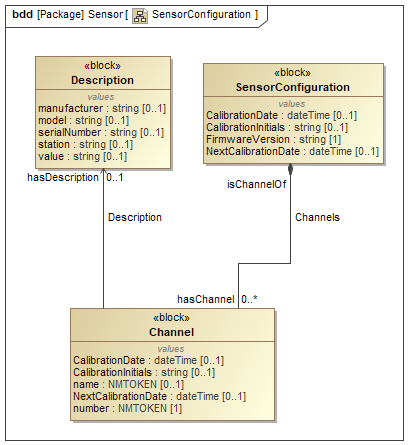
\includegraphics[width=1.0\textwidth]{figures/SensorConfiguration.png}
  \caption{SensorConfiguration Diagram}
  \label{fig:SensorConfiguration}
\end{figure}

\FloatBarrier




\subsubsection{Channel}
\label{sec:Channel}



When \block{Sensor} represents multiple \glspl{sensing element}, each \gls{sensing element} is represented by a \block{Channel} for the \block{Sensor}. 


\paragraph{Attributes of Channel}\mbox{}
\label{sec:Attributes of Channel}

\tbl{Attributes of Channel} lists the attributes of \texttt{Channel}.

\begin{table}[ht]
\centering 
  \caption{Attributes of Channel}
  \label{table:Attributes of Channel}
\tabulinesep=3pt
\begin{tabu} to 6in {|l|l|l|} \everyrow{\hline}
\hline
\rowfont\bfseries {Attribute} & {Type} & {Multiplicity} \\
\tabucline[1.5pt]{}
\property{name}[Channel] & \texttt{NMTOKEN} & 0..1 \\
\property{number}[Channel] & \texttt{NMTOKEN} & 1 \\
\end{tabu}
\end{table}
\FloatBarrier


Descriptions for attributes of \block{Channel}:

\begin{itemize}
\item \property{name}[Channel] : The name of an element or a piece of equipment.
\item \property{number}[Channel] : A unique identifier that will only refer to a specific \gls{sensing element}.
\end{itemize}

\paragraph{Elements of Channel}\mbox{}
\label{sec:Elements of Channel}

\tbl{Elements of Channel} lists the elements of \texttt{Channel}.

\begin{table}[ht]
\centering 
  \caption{Elements of Channel}
  \label{table:Elements of Channel}
\tabulinesep=3pt
\begin{tabu} to 6in {|l|l|l|} \everyrow{\hline}
\hline
\rowfont\bfseries {Element Name} & {Type} & {Multiplicity} \\
\tabucline[1.5pt]{}
\block{CalibrationDate} & \texttt{dateTime} & 0..1 \\
\block{CalibrationInitials} & \texttt{string} & 0..1 \\
\block{NextCalibrationDate} & \texttt{dateTime} & 0..1 \\
\block{Description} & \texttt{Description} & 0..1 \\
\block{Channels} & \texttt{SensorConfiguration} & 1 \\
\end{tabu}
\end{table}
\FloatBarrier


Descriptions for elements of \block{Channel}:

\begin{itemize}
\item \block{CalibrationDate} : Date upon which the \gls{sensor unit} was last calibrated to the \gls{sensor element}.
\item \block{CalibrationInitials} : The initials of the person verifying the validity of the calibration data.
\item \block{NextCalibrationDate} : Date upon which the \gls{sensor element} is next scheduled to be calibrated with the \gls{sensor unit}.

\item \block{Description} : The descriptive content.
\item \block{Channels} : \block{Channels} \glspl{organize} \block{Channel} elements.

\end{itemize}
\FloatBarrier

\subsubsection{SensorConfiguration}
\label{sec:SensorConfiguration}



\block{SensorConfiguration} contains configuration information about a \block{Sensor}.


\paragraph{Elements of SensorConfiguration}\mbox{}
\label{sec:Elements of SensorConfiguration}

\tbl{Elements of SensorConfiguration} lists the elements of \texttt{SensorConfiguration}.

\begin{table}[ht]
\centering 
  \caption{Elements of SensorConfiguration}
  \label{table:Elements of SensorConfiguration}
\tabulinesep=3pt
\begin{tabu} to 6in {|l|l|l|} \everyrow{\hline}
\hline
\rowfont\bfseries {Element Name} & {Type} & {Multiplicity} \\
\tabucline[1.5pt]{}
\block{CalibrationDate} & \texttt{dateTime} & 0..1 \\
\block{CalibrationInitials} & \texttt{string} & 0..1 \\
\block{FirmwareVersion} & \texttt{string} & 1 \\
\block{NextCalibrationDate} & \texttt{dateTime} & 0..1 \\
\block{Channels} & \texttt{Channel} & 0..* \\
\end{tabu}
\end{table}
\FloatBarrier


Descriptions for elements of \block{SensorConfiguration}:

\begin{itemize}
\item \block{CalibrationDate} : Date upon which the \gls{sensor unit} was last calibrated.
\item \block{CalibrationInitials} : The initials of the person verifying the validity of the calibration data.
\item \block{FirmwareVersion} : Version number for the sensor unit as specified by the manufacturer.

\item \block{NextCalibrationDate} : Date upon which the \gls{sensor unit} is next scheduled to be calibrated.
\item \block{Channels} : \block{Channels} \glspl{organize} \block{Channel} elements.

\end{itemize}
\FloatBarrier
